\documentclass[11pt, oneside]{article}   	% use "amsart" instead of "article" for AMSLaTeX format
\usepackage{geometry}                		% See geometry.pdf to learn the layout options. There are lots.
\geometry{letterpaper}                   		% ... or a4paper or a5paper or ... 
%\geometry{landscape}                		% Activate for rotated page geometry
%\usepackage[parfill]{parskip}    		% Activate to begin paragraphs with an empty line rather than an indent
\usepackage{graphicx}				% Use pdf, png, jpg, or eps§ with pdflatex; use eps in DVI mode
								% TeX will automatically convert eps --> pdf in pdflatex		
\usepackage{amssymb}
\usepackage{hyperref}
\usepackage{float}

\usepackage{listings}
\usepackage{xcolor}
\usepackage{dirtytalk}

\definecolor{codegreen}{rgb}{0,0.6,0}
\definecolor{codegray}{rgb}{0.5,0.5,0.5}
\definecolor{codepurple}{rgb}{0.58,0,0.82}
\definecolor{backcolour}{rgb}{0.95,0.95,0.92}

\lstdefinestyle{mystyle}{
    backgroundcolor=\color{backcolour},   
    commentstyle=\color{codegreen},
    keywordstyle=\color{magenta},
    numberstyle=\tiny\color{codegray},
    stringstyle=\color{codepurple},
    basicstyle=\ttfamily\footnotesize,
    breakatwhitespace=false,         
    breaklines=true,                 
    captionpos=b,                    
    keepspaces=true,                 
    numbers=left,                    
    numbersep=5pt,                  
    showspaces=false,                
    showstringspaces=false,
    showtabs=false,                  
    tabsize=2
}

\lstset{style=mystyle}



%SetFonts

%SetFonts


\title{Part 1}
\author{Yapi Donatien Achou}
%\date{}							% Activate to display a given date or no date

\begin{document}
\maketitle

\section{Optimising a python script to leverage multicore}
In this use case, a python script processing millions of records runs on a single thread. The question is, how can we leverage multicore to improve the execution time.\\
\\
\say{A thread of execution is the smallest sequence of programmed instructions that can be managed independently by a scheduler, which is typically a part of the operating system. In many cases, a thread is a component of a process.}, \cite{threads}, as shown in Figure \ref{fig:threads}

\begin{figure}[H] %  figure placement: here, top, bottom, or page
   \centering
   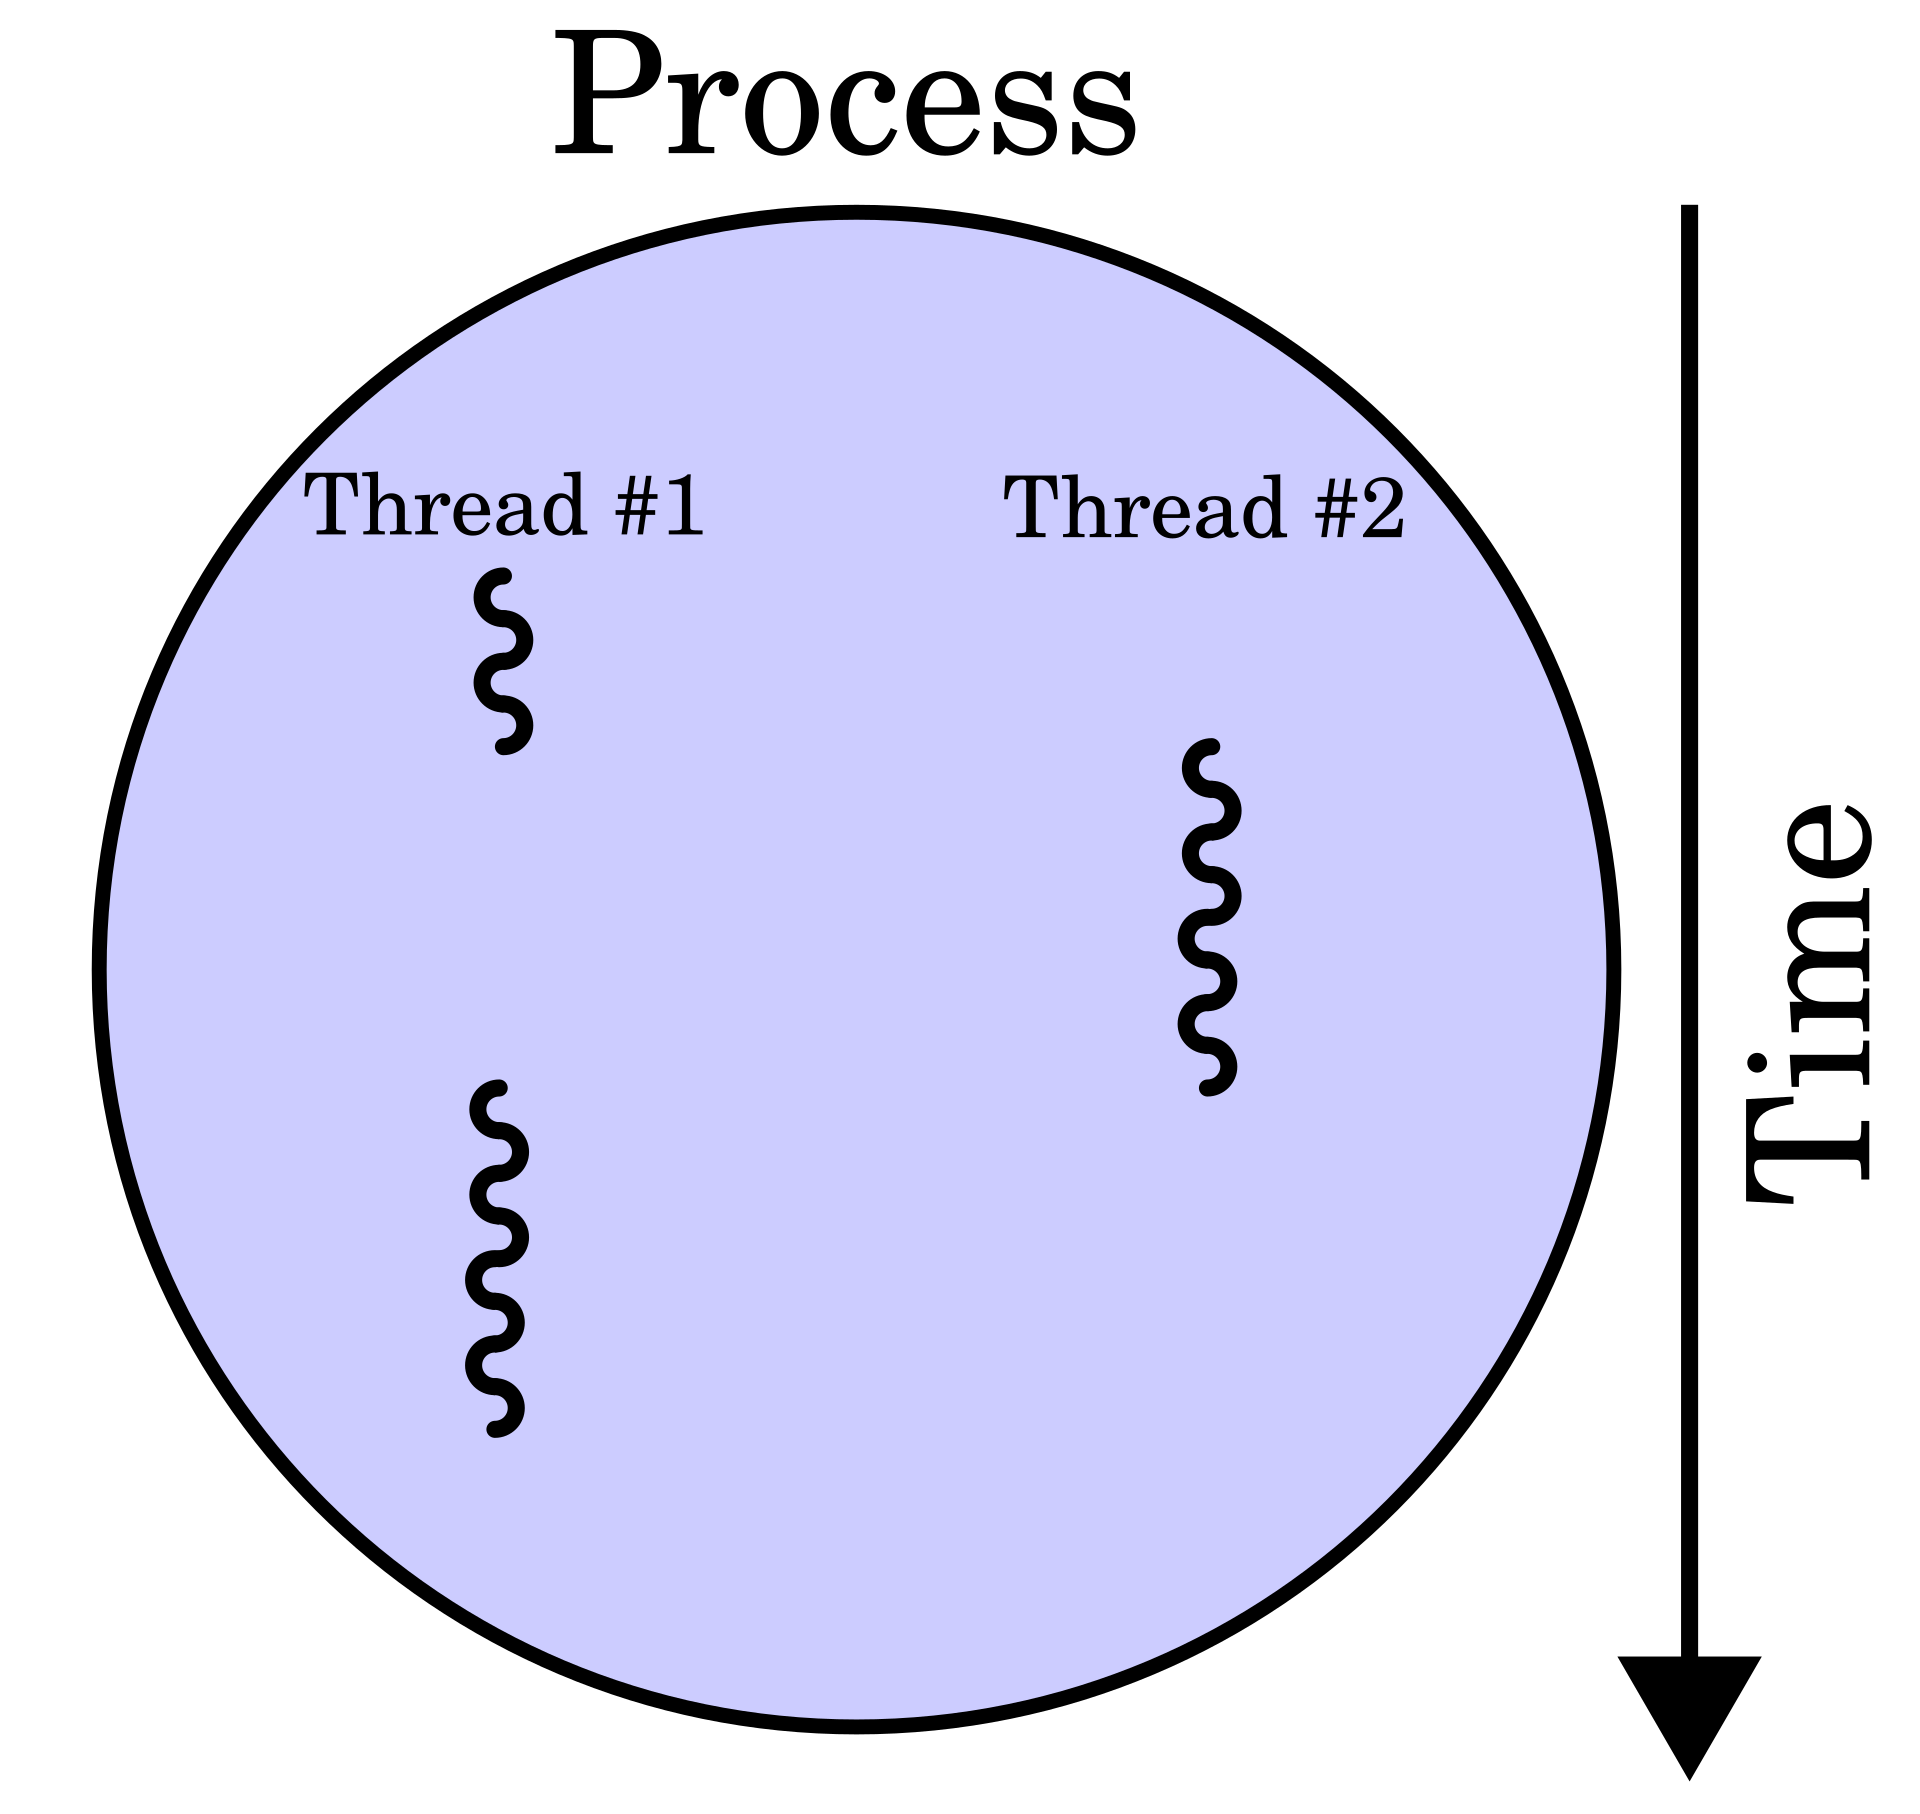
\includegraphics[width=2in]{images/threads.png} 
   \caption{Threads in a process. Curtesy Wikipedia, \cite{threads}}
   \label{fig:threads}
\end{figure}

Since in this case the script uses only a single thread to process millions of records, it makes  sens to distribute the computational load accros multiple threads within one or more processes in order to improve execution time.\\
\\
As opposed to a thread, a process has its own resource (memory, computational unit) and \say{each CPU (core) executes a single process at a time}, \cite{process}, so to improve execution time we can use multiple processes on a multicore architecture machine. In addition, processing millions of records is a CPU intensive task and processes shine in these king of tasks.\\
\\
In Python parallelism can be achieved by using the \textbf{multiprocessing} module. We can use the \textbf{Pool} object in the multiprocessing module to distribute the input records across processes and achieve \textbf{data parallelism}, \cite{multiprocess}. The \textbf{Pool} object creates multiples processes each running independently and leveraging multiples cpu cores. \\
\\

Figure \ref{fig:para} shows the implementation of a function that uses the multiprocessing python module to achieve data parallelism using the Pool object, while Figure \ref{fig:execute} show the different execution time, with different records size.

\begin{figure}[H] %  figure placement: here, top, bottom, or page
   \centering
   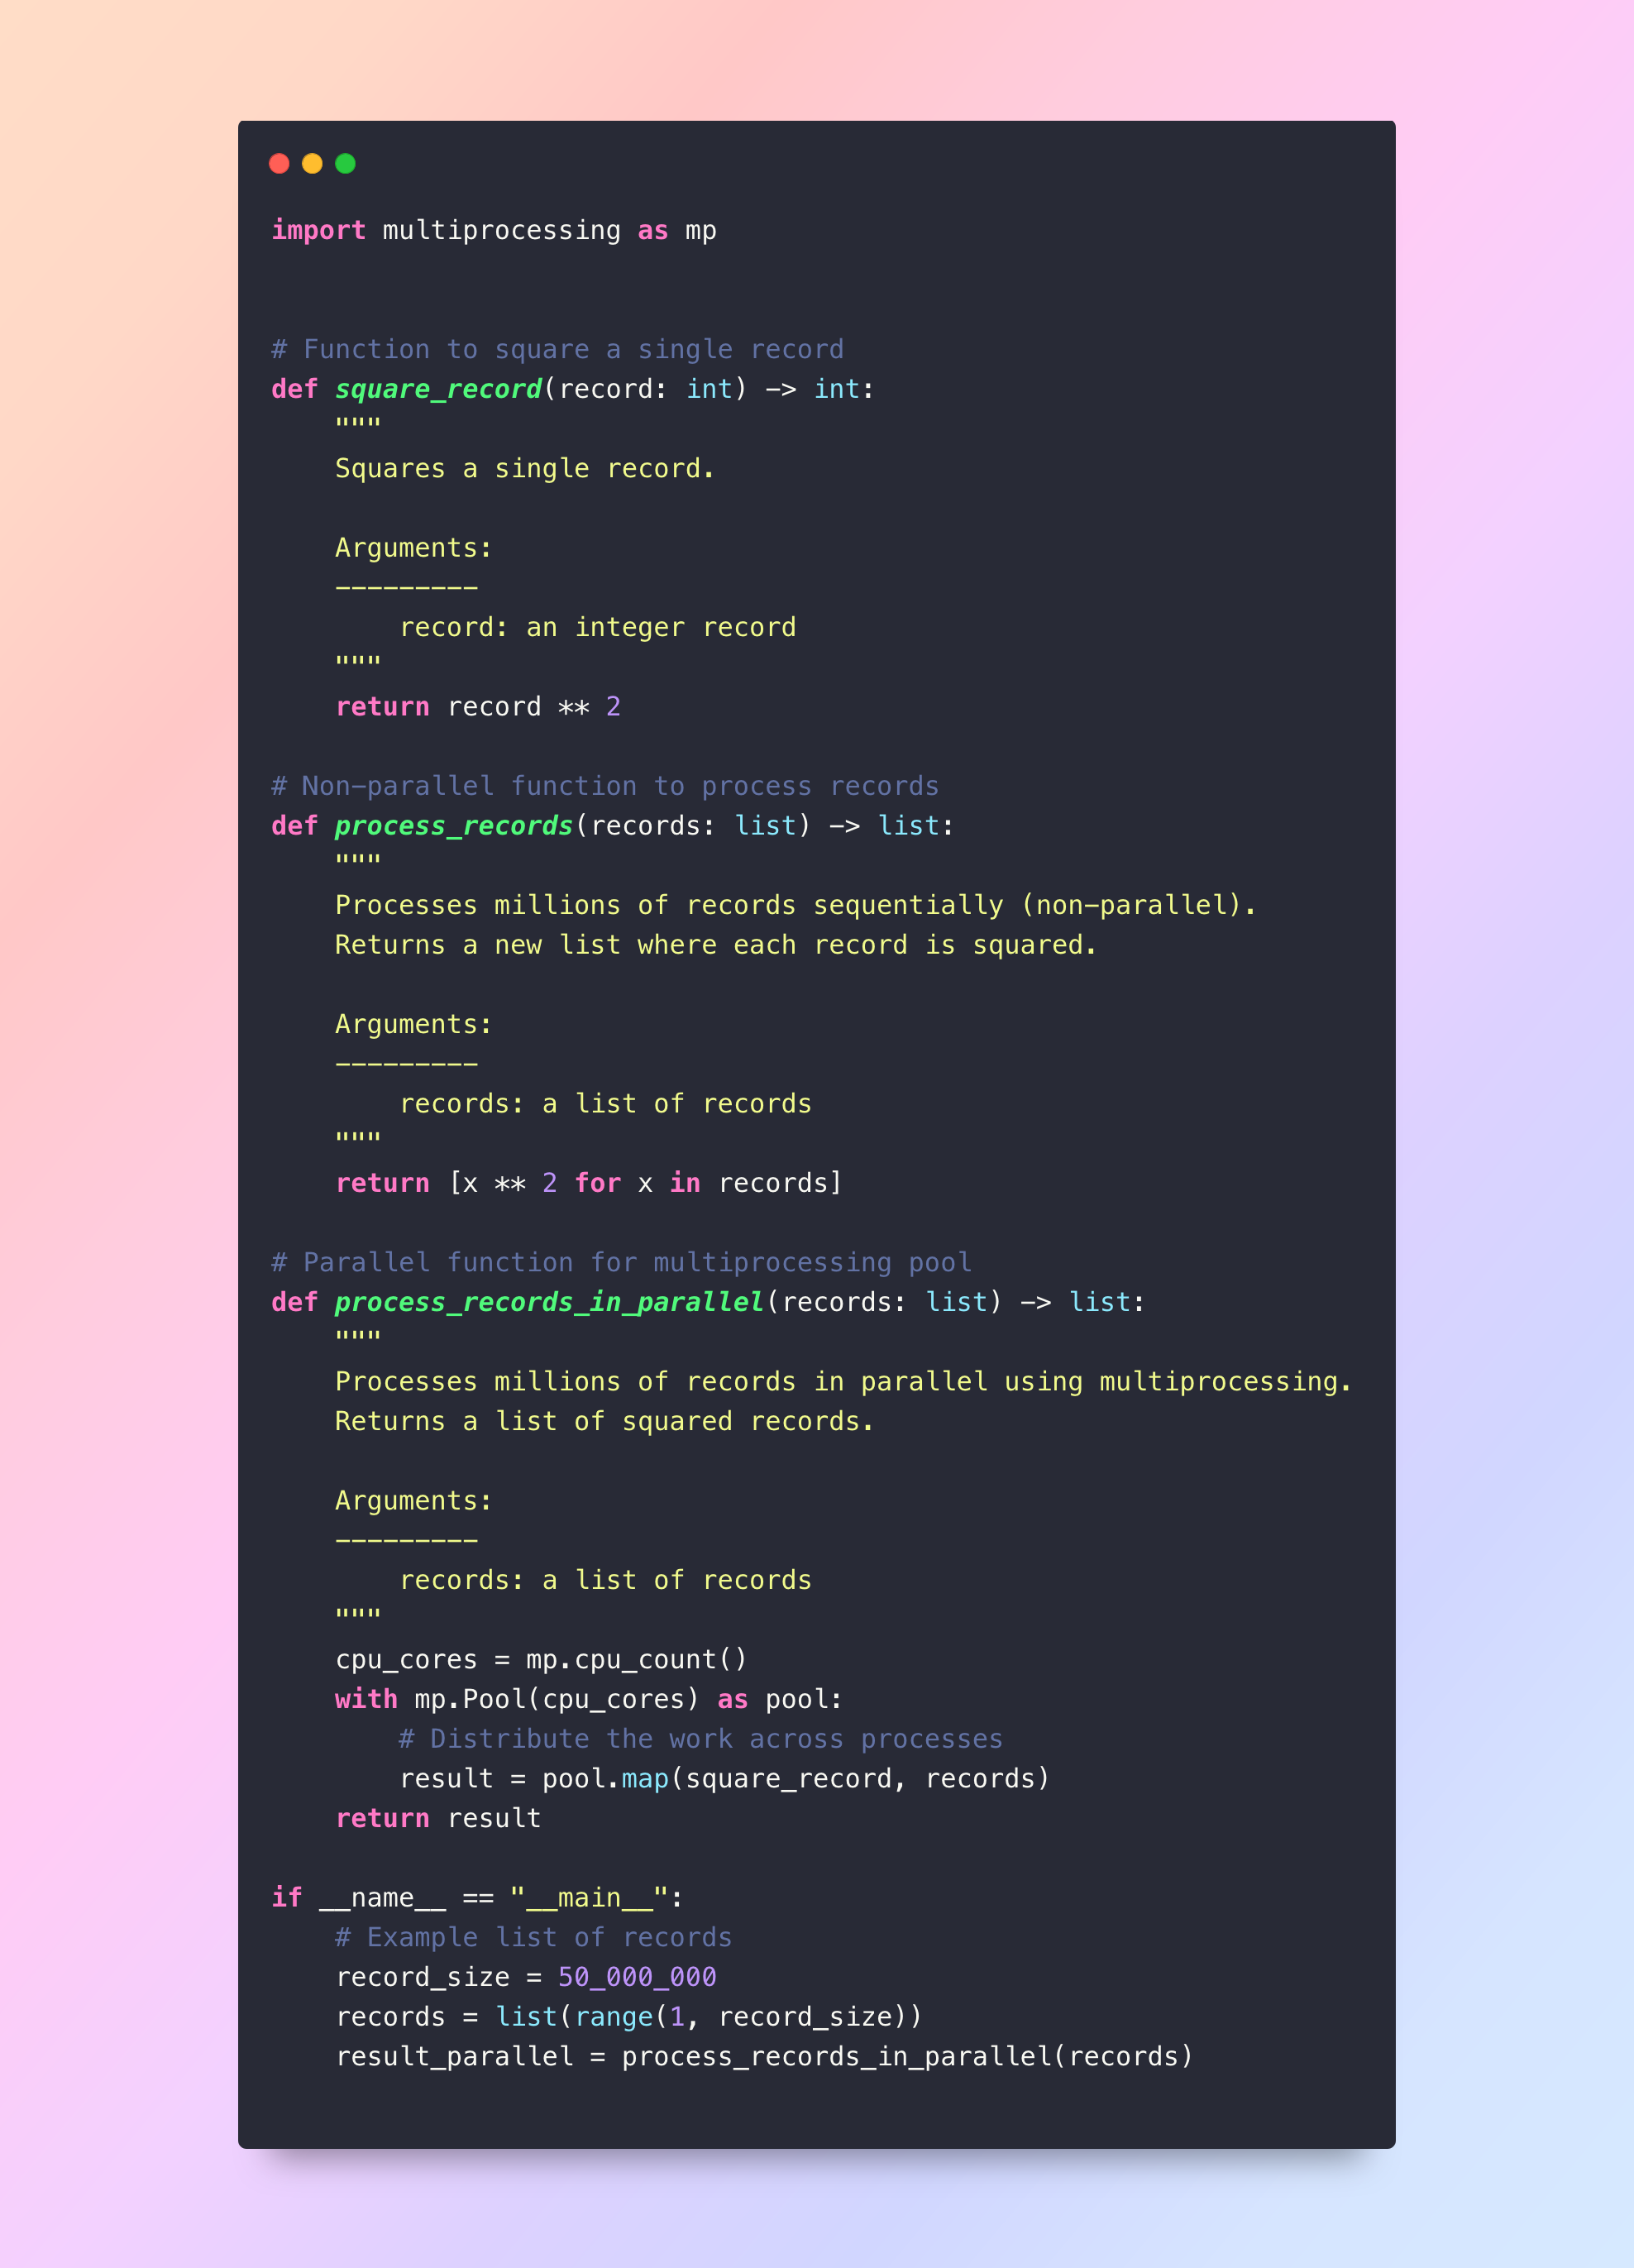
\includegraphics[width=4in]{images/para_code} 
   \caption{Parallelism of a function using multiprocessing module in Python}
   \label{fig:para}
\end{figure}

\begin{figure}[H] %  figure placement: here, top, bottom, or page
   \centering
   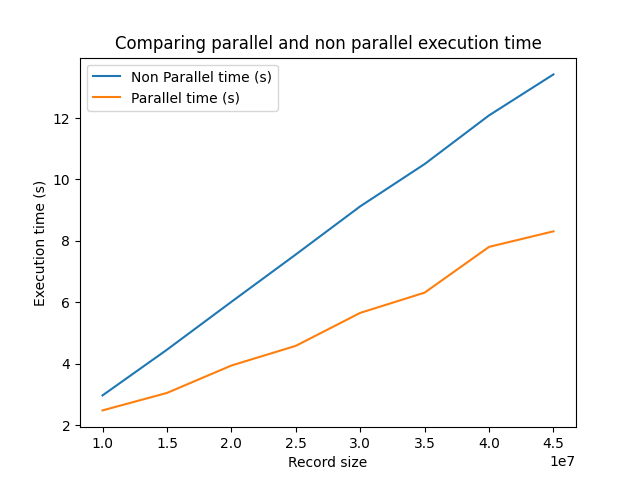
\includegraphics[width=4in]{images/compare} 
   \caption{Execution time of a single thread vs a multi process code}
   \label{fig:execute}
\end{figure}




\section{Handling invalid data format in azure Data Factory}
Data format can refer to constraints placed upon the interpretation of data in a type system (data type), a format for encoding data for storage in a computer file (file format), \cite{wiki}.\\
\\
Inconsistency between data type and file format between data in a data lake source and a dataset in Azure Data Factory can cause an invalid data format error in a pipeline run. For illustration purpose we will be focusing on a file format invalid data format error.\\
\\
A data pipeline failure due to an invalid data format in Azure Data Factory can occur, for example, when there is a mismatch between the format of the source data (e.g., in an Azure Data Lake container) and the source dataset configuration in Azure Data Factory.\\
\\
Let’s say the source data in the Azure Data Lake container is in CSV format, but when configuring the dataset in Azure Data Factory, we mistakenly set the dataset format to JSON. This mismatch would cause the pipeline to fail, as Azure Data Factory would try to interpret the CSV file as JSON, leading to this case in a JsonInvalidDataFormat error.\\
\\
I have reproduced this error by:
\begin{itemize}
        \item Provisioning a storage account and populated a source container with csv files. See Figure \ref{fig:storage}
        \item Provisioning an Azure Data Factory resource
        \item Creating a source linked service
        \item Creating a sink linked service
        \item Creating a JSON source Dataset. See Figure \ref{fig:sourceDataset}
        \item Creating a CSV sink Dataset. See Figure \ref{fig:sinkDataset}
        \item Creating a copy pipeline from source to sink. See Figure \ref{fig:pipeline_config}
          \item running the pipeline to reproduce the error
\end{itemize}
\begin{figure}[H] %  figure placement: here, top, bottom, or page
   \centering
   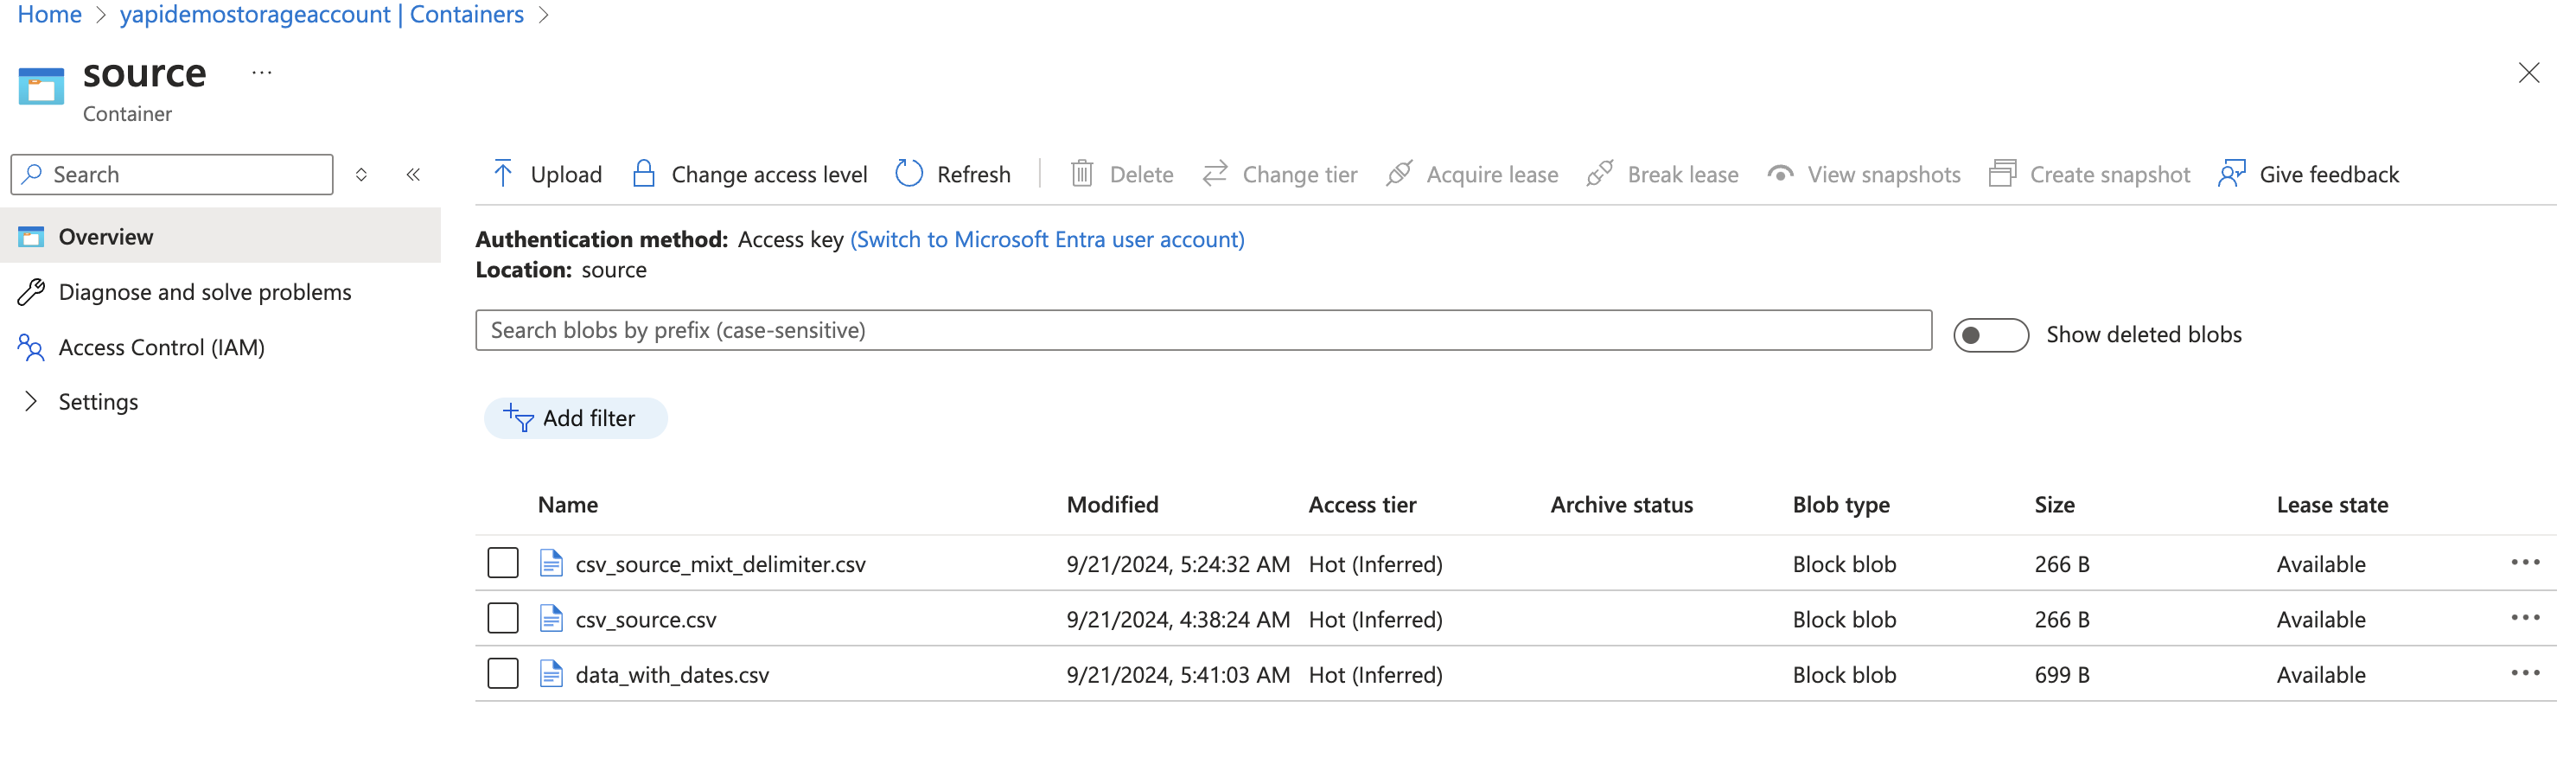
\includegraphics[width=6in]{images/storage.png} 
   \caption{Azure source container with CSV files }
   \label{fig:storage}
\end{figure}

\begin{figure}[H] %  figure placement: here, top, bottom, or page
   \centering
   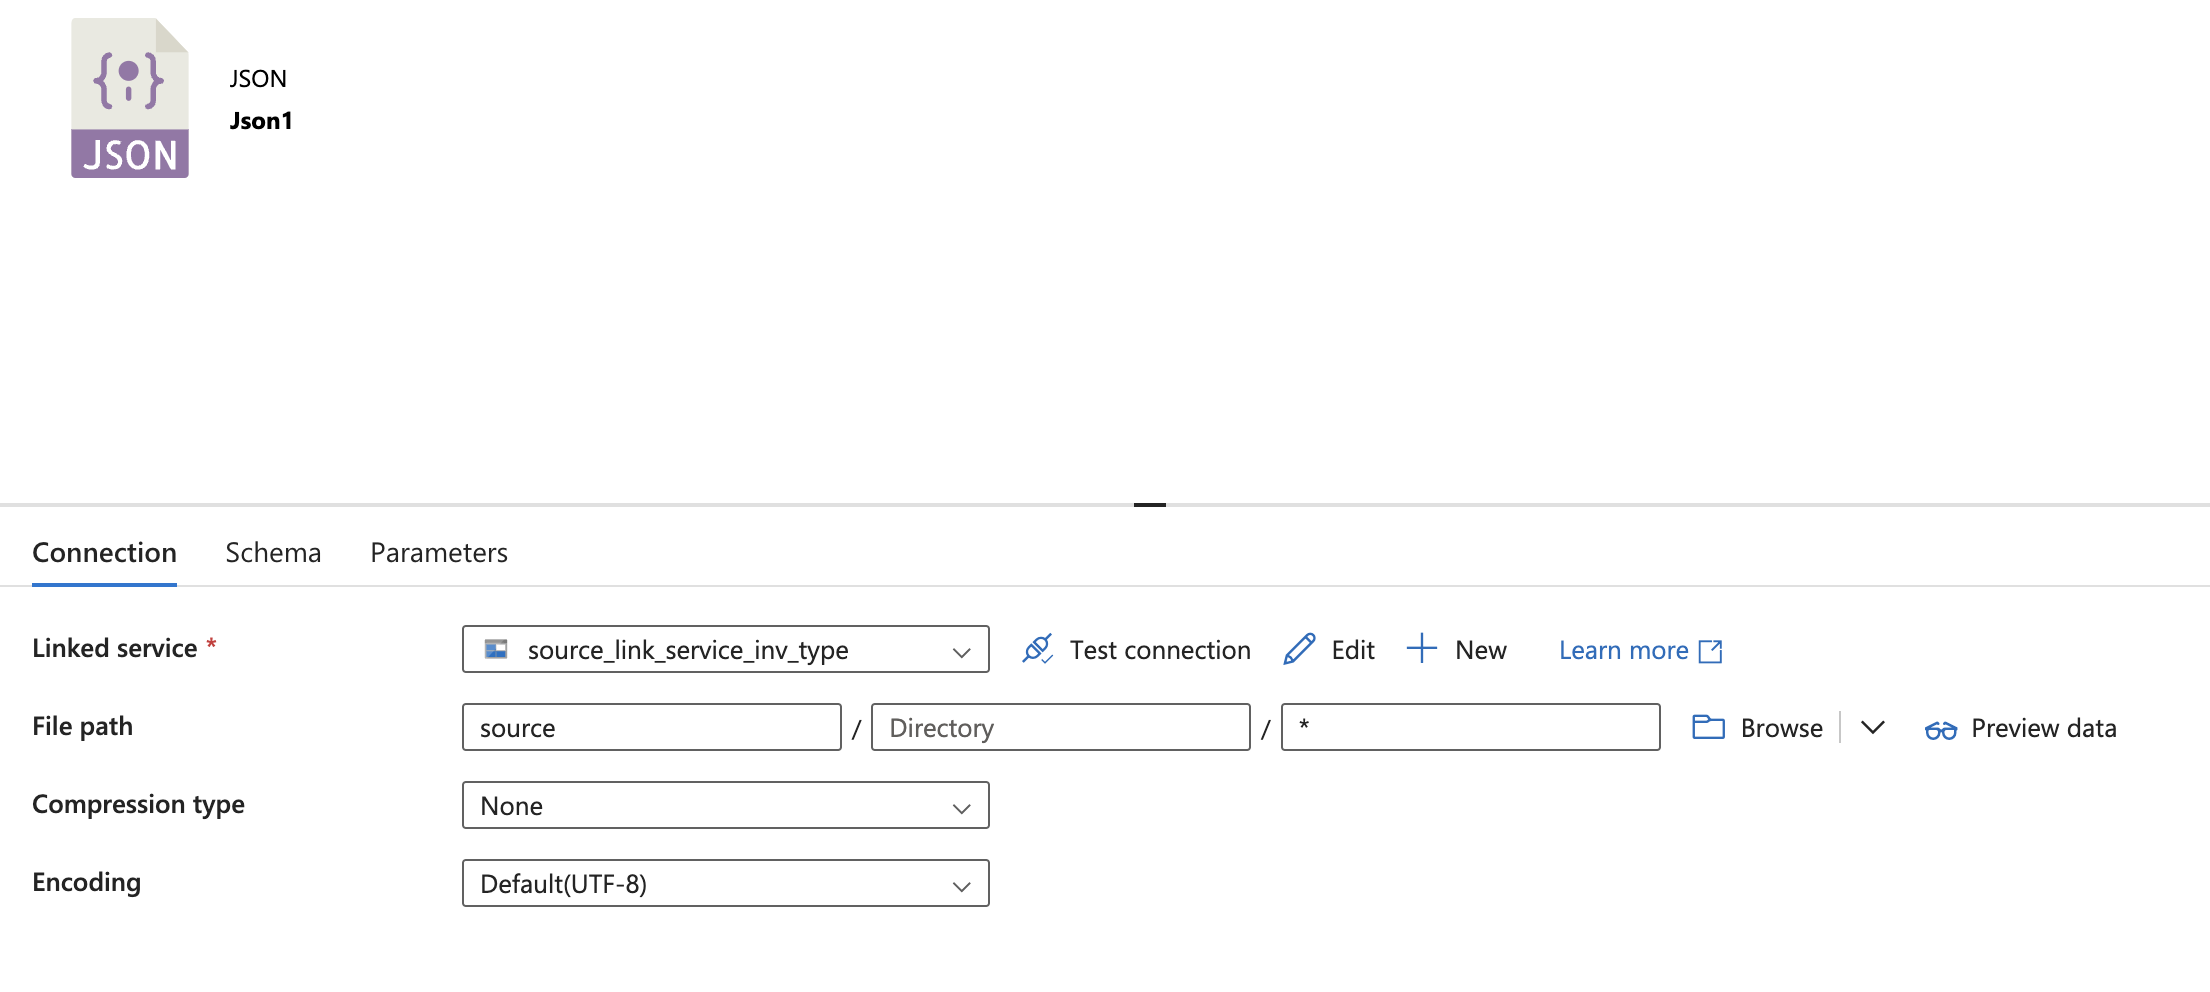
\includegraphics[width=6in]{images/sourceDataset.png} 
   \caption{Azure Data Factory source JSON Dataset}
   \label{fig:sourceDataset}
\end{figure}

\begin{figure}[H] %  figure placement: here, top, bottom, or page
   \centering
   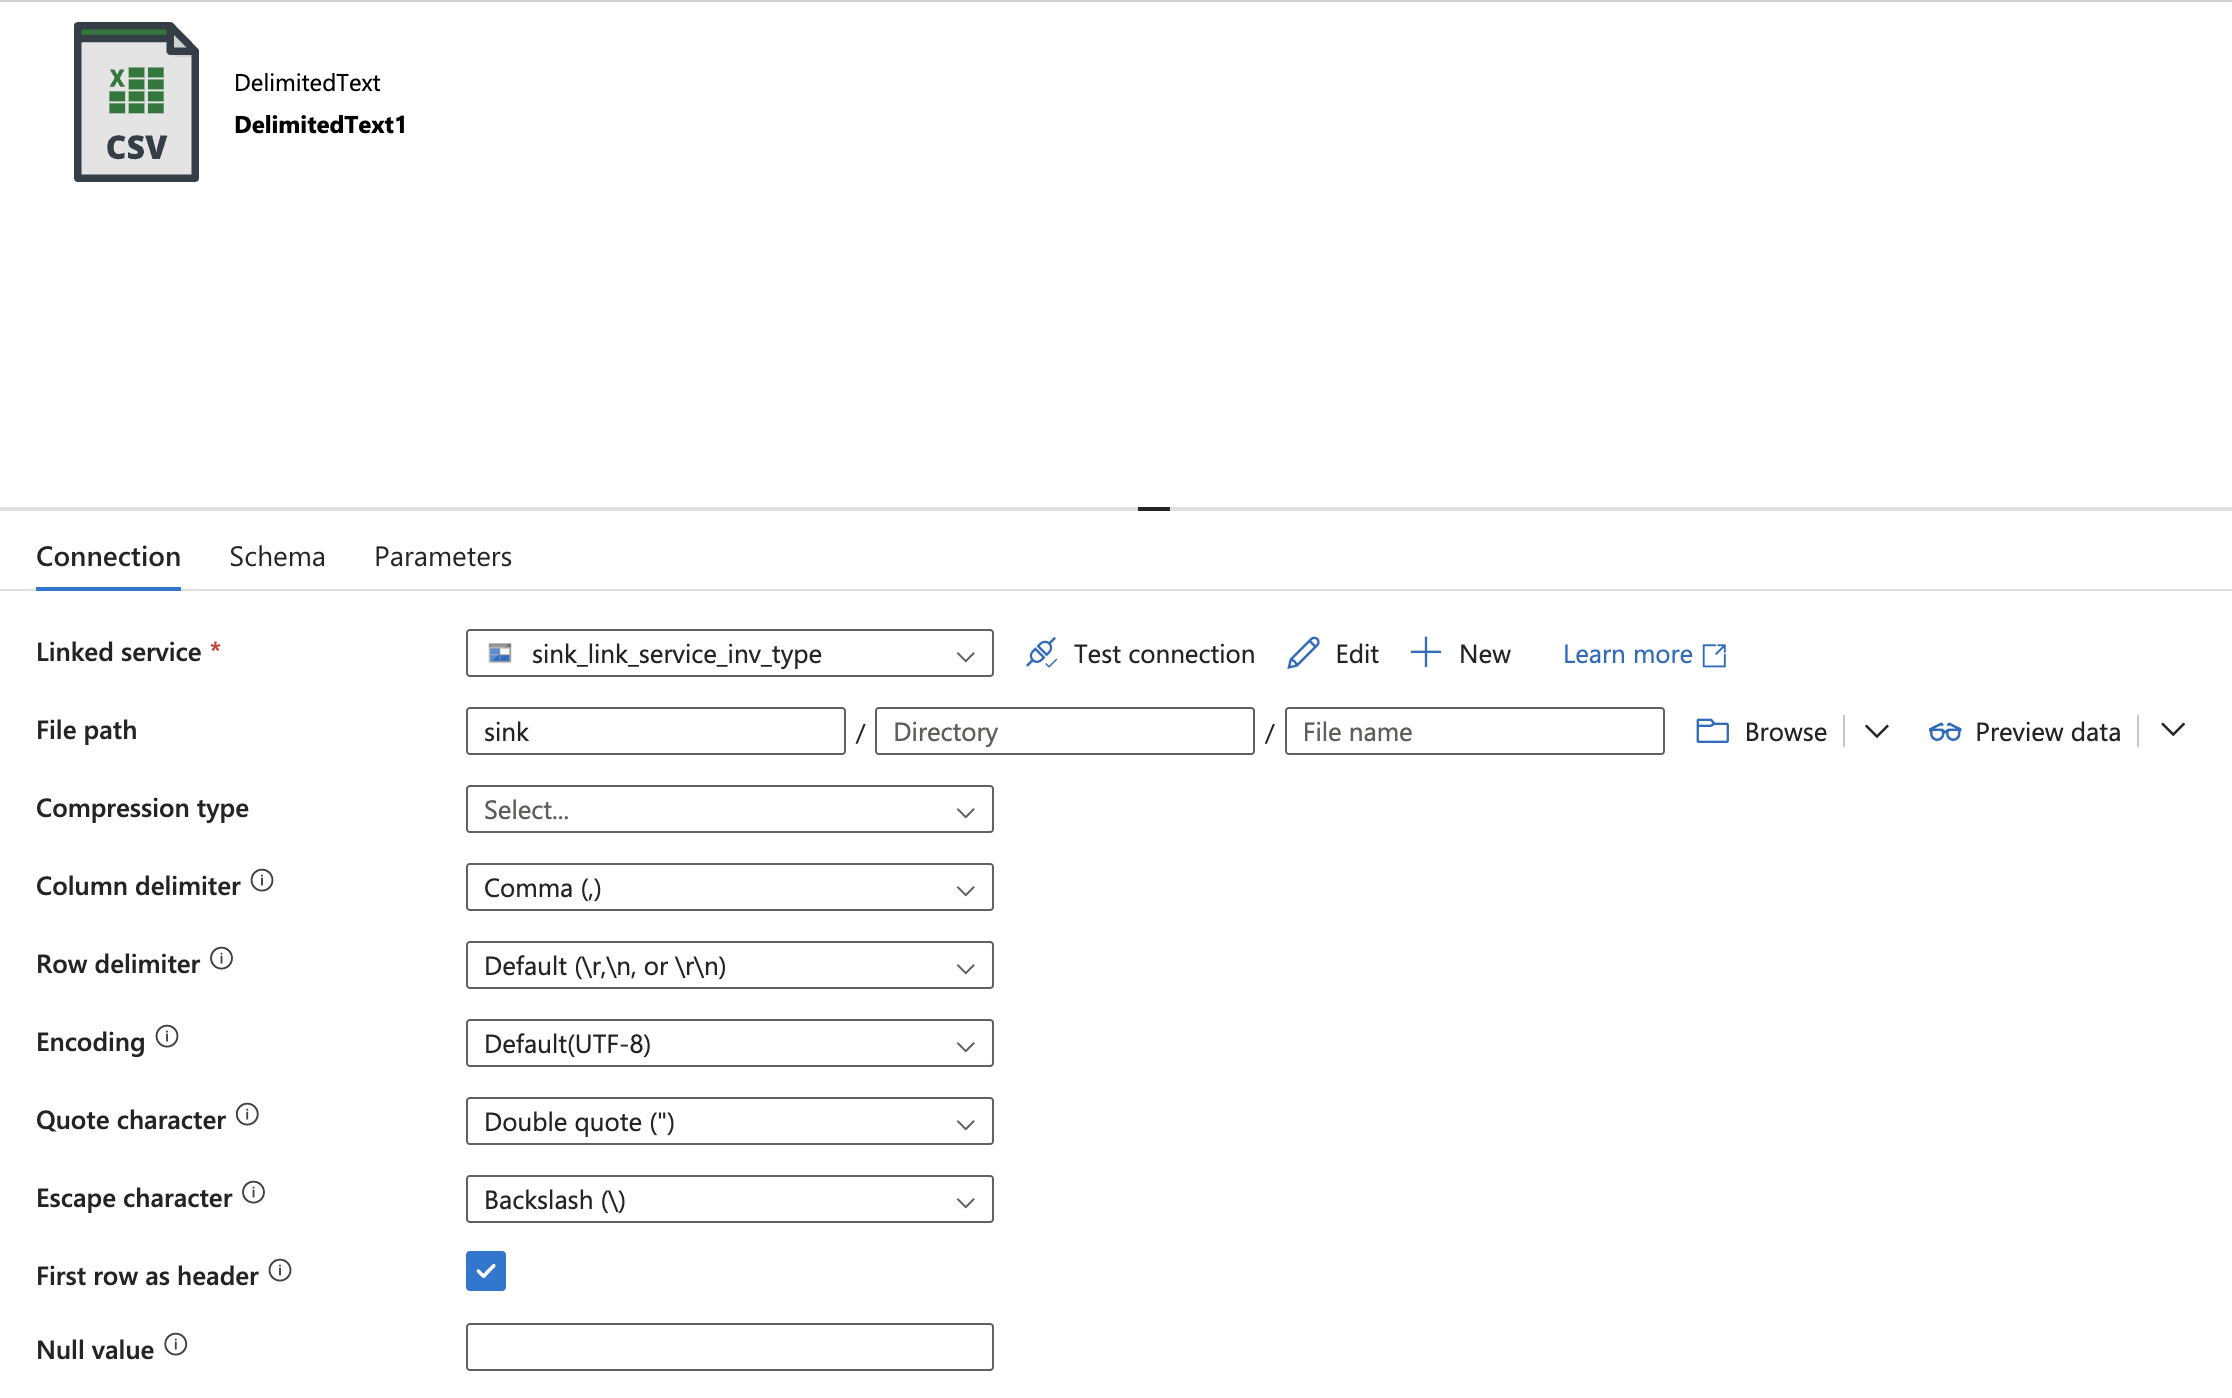
\includegraphics[width=6in]{images/sinkDataset.png} 
   \caption{Azure Data Factory sink CSV Dataset}
   \label{fig:sinkDataset}
\end{figure}

\begin{figure}[H] %  figure placement: here, top, bottom, or page
   \centering
   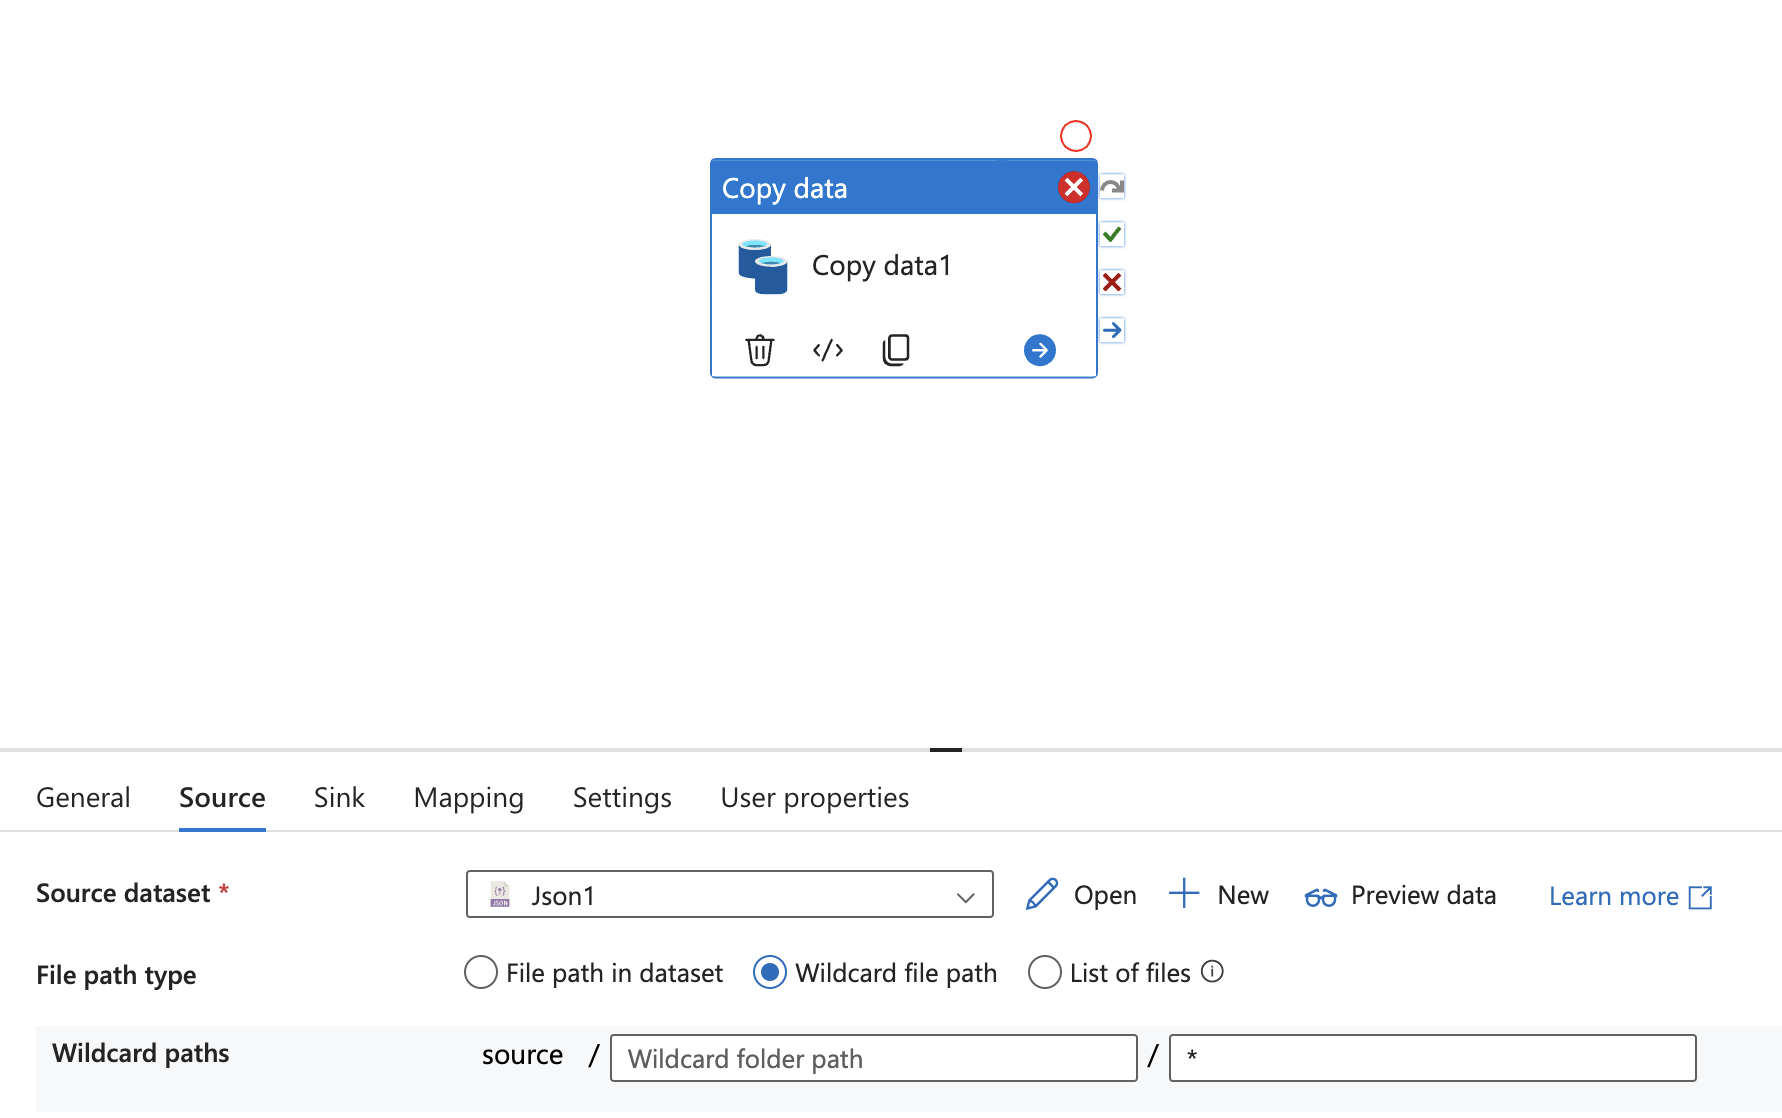
\includegraphics[width=6in]{images/pipeline_config.png} 
   \caption{Azure Data Factory Copy pipeline configuration}
   \label{fig:pipeline_config}
\end{figure}



 The pipeline  failed with a JsonInvalidDataFormat as see in figure \ref{fig:error}
 \begin{figure}[H] %  figure placement: here, top, bottom, or page
   \centering
   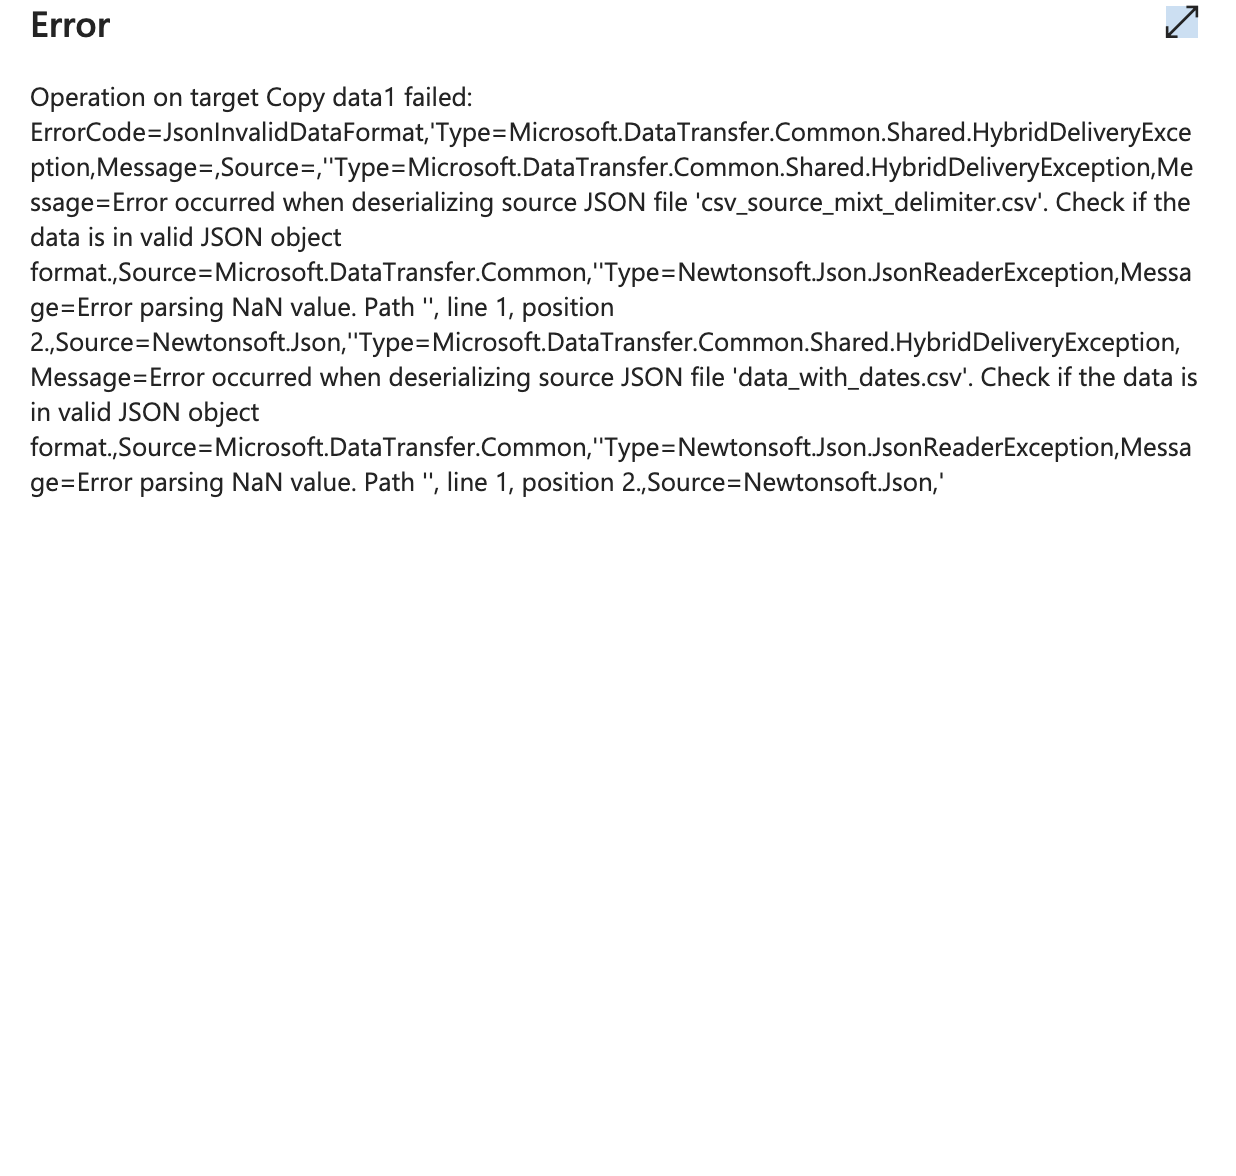
\includegraphics[width=6in]{images/error.png} 
   \caption{JsonInvalidDataFormat error}
   \label{fig:error}
\end{figure}


\subsection{Debugging such error in Azure Data Factory}
The First approach in debugging this issue is by
\begin{enumerate}
        \item Carefully reading the error message for clues in finding the cause
          \item Verifying that the dataset in Azure Data Factory configurations (data format) matches the format of the source data ( files located in Azure data lake container for example)
\end{enumerate}
In this case the error message clearly says that there is a difference between the source files  format in the Azure data lake container and the configured Dataset format in Azure Data Factory.
To fix the issue:
\begin{enumerate}
        \item Create a new Dataset that matches the format of the files in the source Azure container in this case CSV. See Figure \ref{fig:dataset2}
          \item Update the pipeline configuration to take the new Dataset as source. See Figure  \ref{fig:pipeline2}
\end{enumerate}

\begin{figure}[H] %  figure placement: here, top, bottom, or page
   \centering
   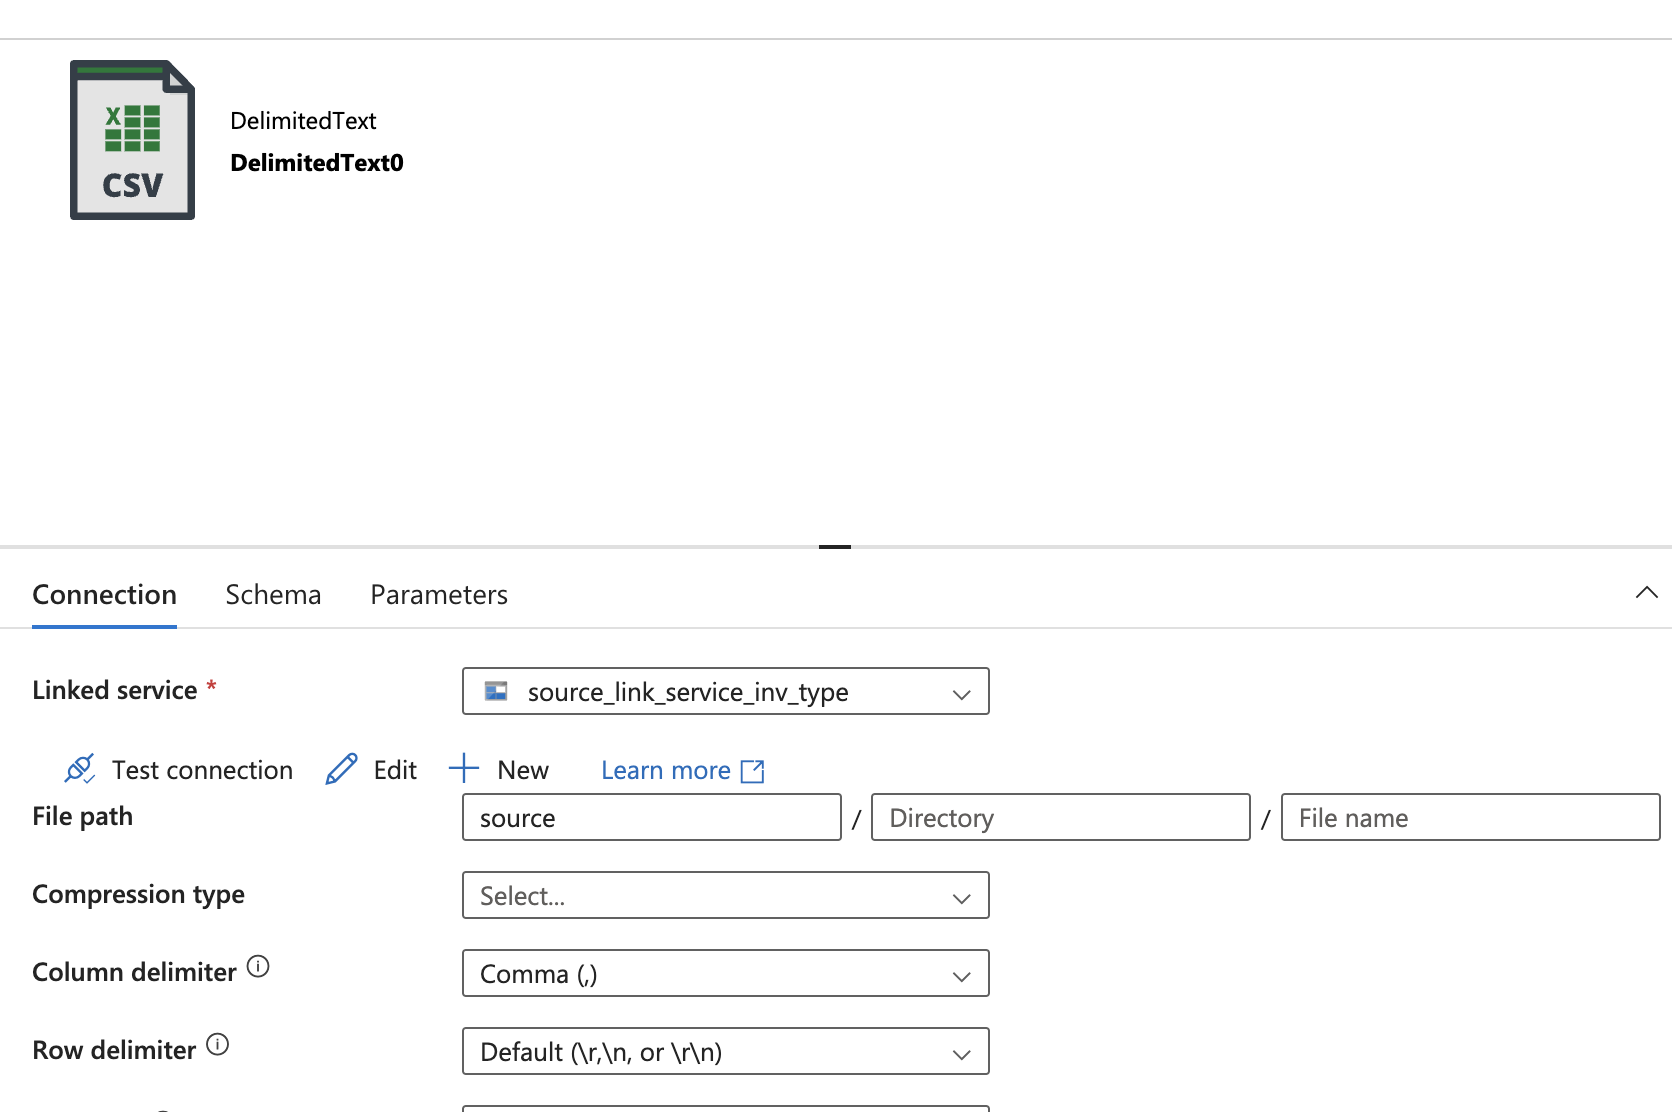
\includegraphics[width=6in]{images/source2.png} 
   \caption{Azure Data Factory source CSV Dataset}
   \label{fig:dataset2}
\end{figure}

\begin{figure}[H] %  figure placement: here, top, bottom, or page
   \centering
   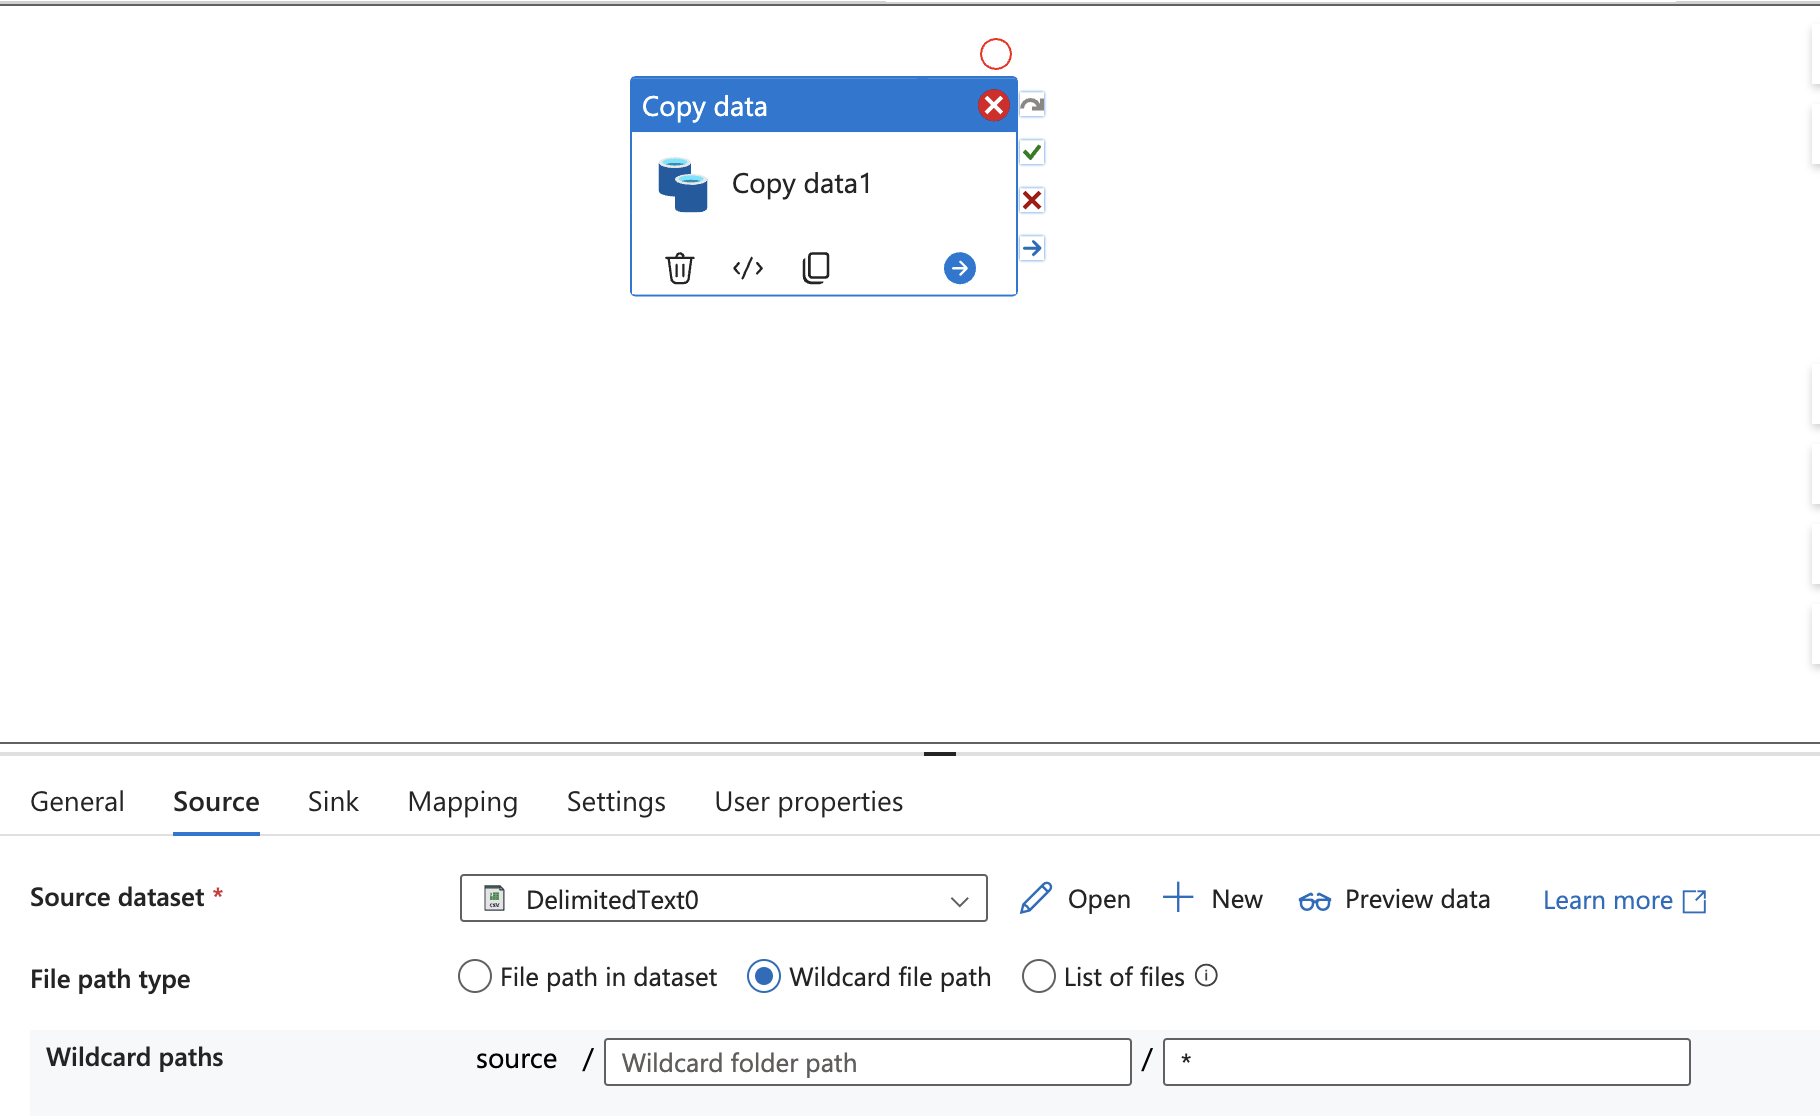
\includegraphics[width=6in]{images/pipeline2} 
   \caption{Azure Data Factory updated pipeline}
   \label{fig:pipeline2}
\end{figure}

After taking these measures the pipeline runs successfully  as seen in Figure \ref{fig:success}
\begin{figure}[H] %  figure placement: here, top, bottom, or page
   \centering
   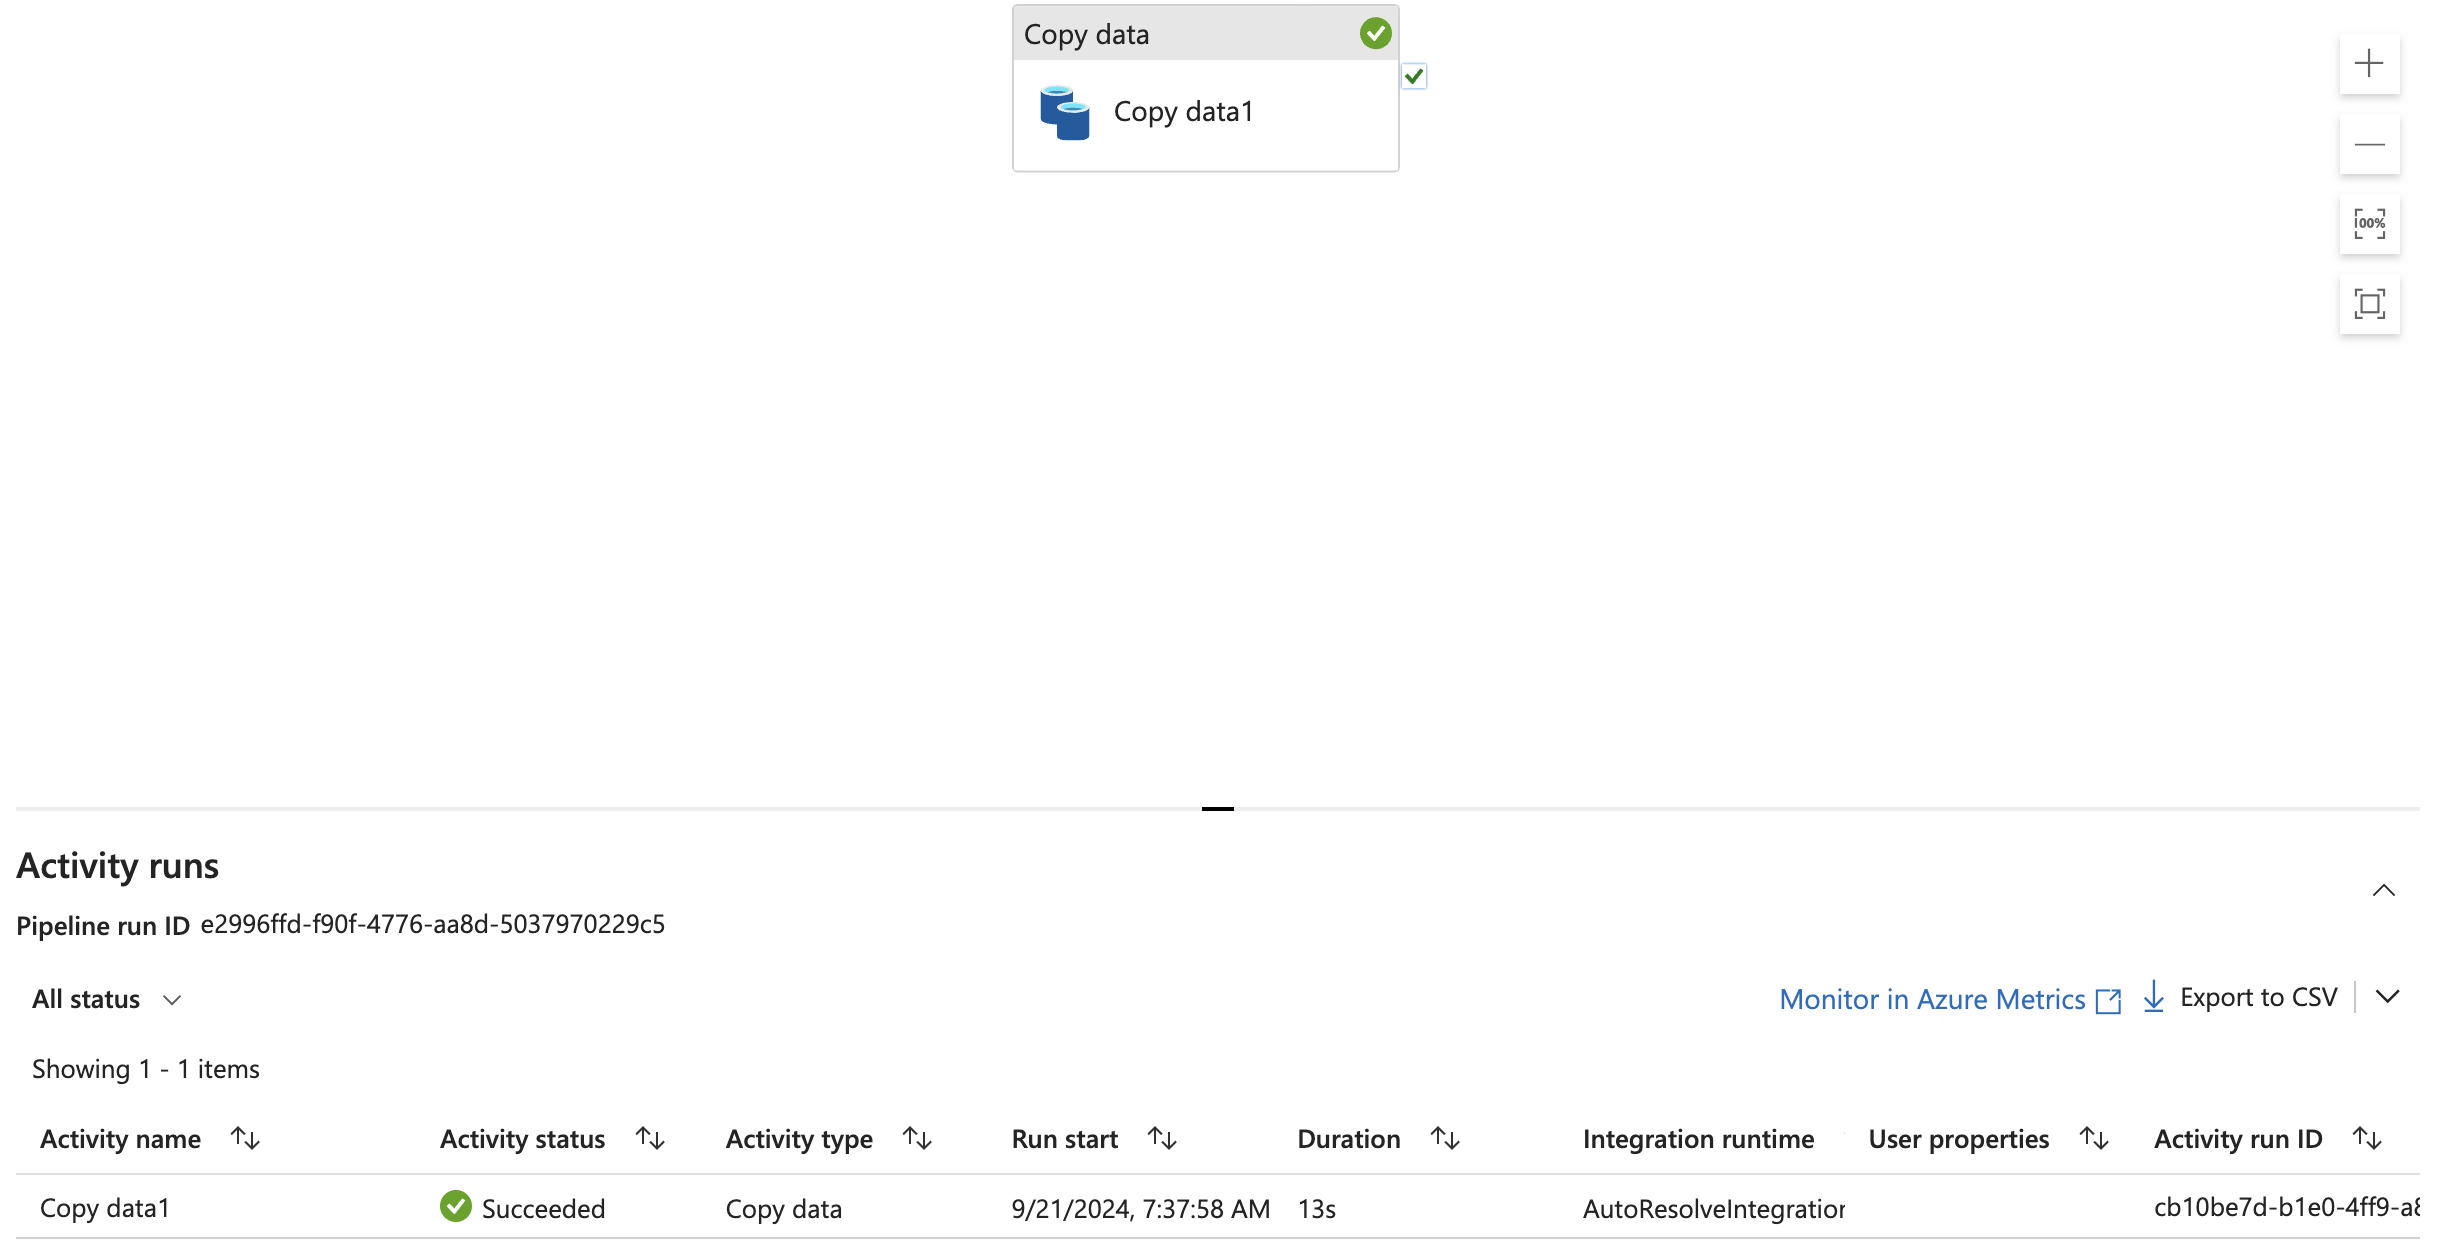
\includegraphics[width=6in]{images/success} 
   \caption{Azure Data Factory successful data copy}
   \label{fig:success}
\end{figure}






\subsection{Making sure it can be avoided in the future}
In general, it is a good idea to validate \cite{validation}, and test your data pipeline before deployment. Validation can be done by setting up data quality contraints during pipeline development.\\
\\
Testing can be achieved by using debugging tools available in Azure Data Factory, \cite{debugtool}\\
\\
In this particular case proper approaches to avoid data format error in the future:
\begin{itemize}
\item Debugging the pipeline by pressing the Debug button in the pipeline creation menue. This will reveal any issue before running the pipeline
   \item Add a validation activity in the pipeline by validating the source dataset before the pipeline is run \cite{validation}. This will ensure that the pipeline only runs after the validation is passed. See Figure \ref{fig:validation}
   \item Use Azure Data factory Dataflow \cite{dataflow}, for a more detailed and thorough data validation. This will allow for data type validation, schema validation, and more in depth data format validation. See Figure \ref{fig:dataflow}
\end{itemize}

\begin{figure}[H] %  figure placement: here, top, bottom, or page
   \centering
   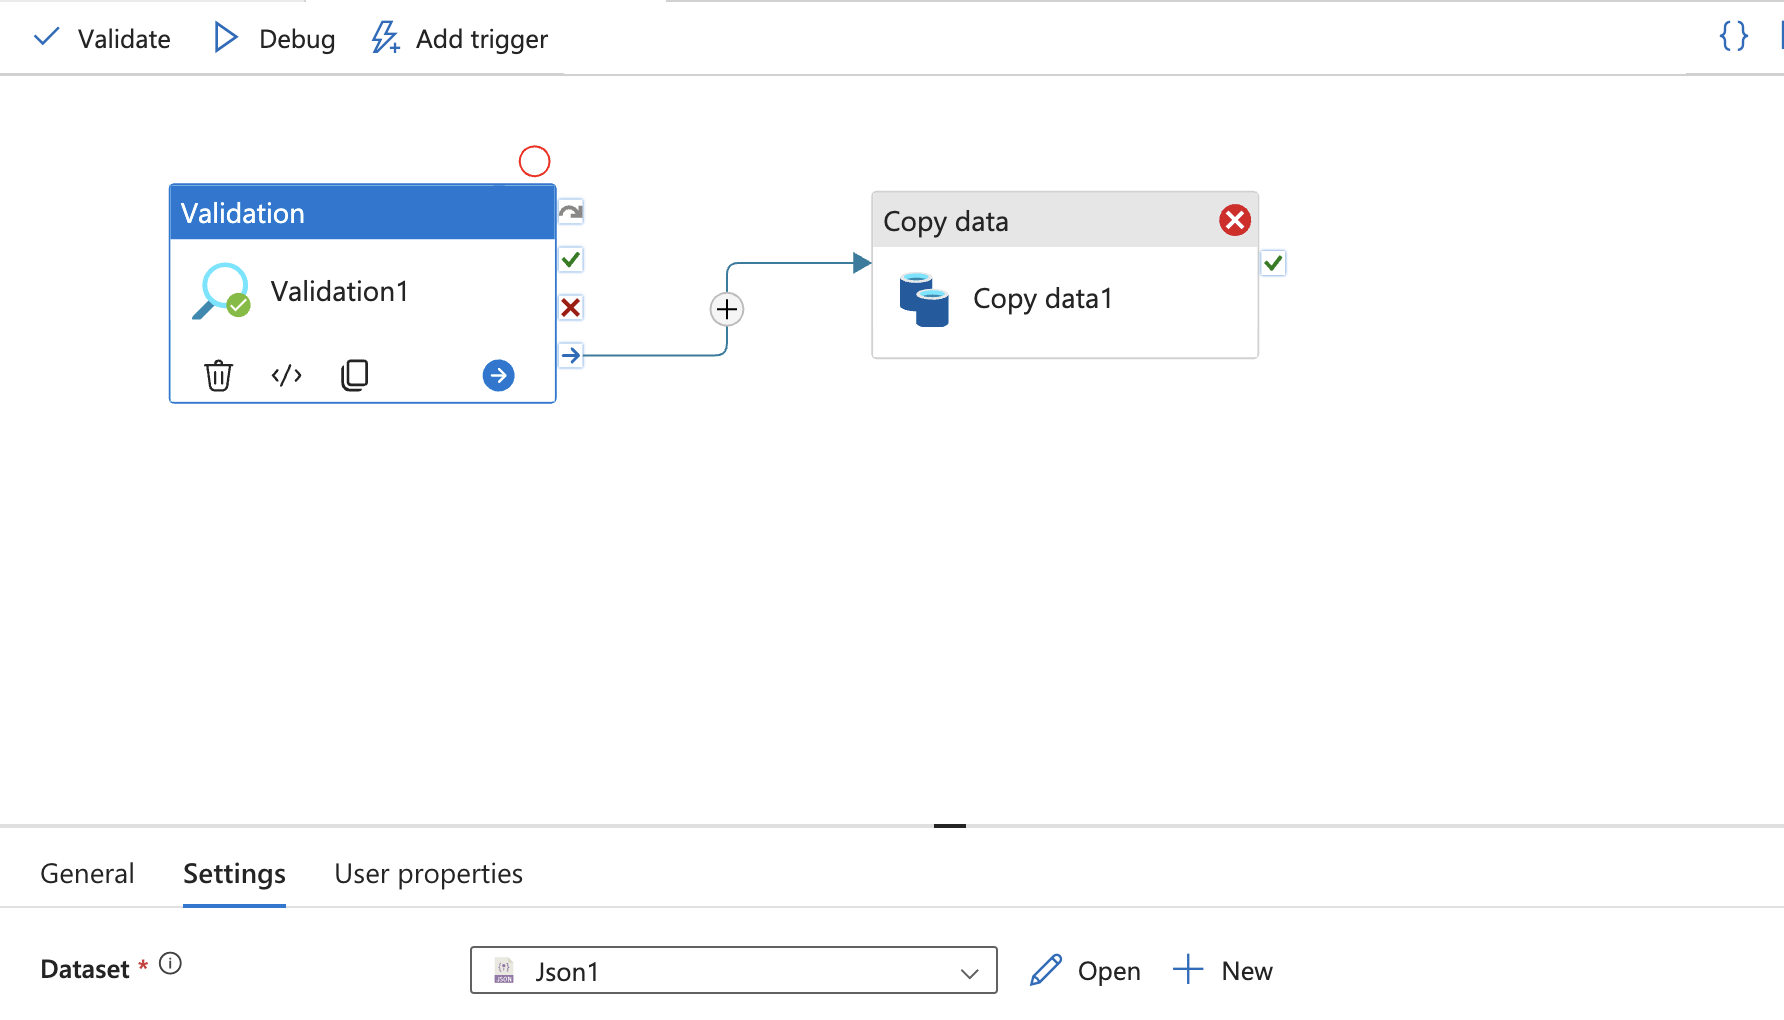
\includegraphics[width=6in]{images/validation} 
   \caption{Validation activity attached to the source dataset in a copy pipeline}
   \label{fig:validation}
\end{figure}

\begin{figure}[H] %  figure placement: here, top, bottom, or page
   \centering
   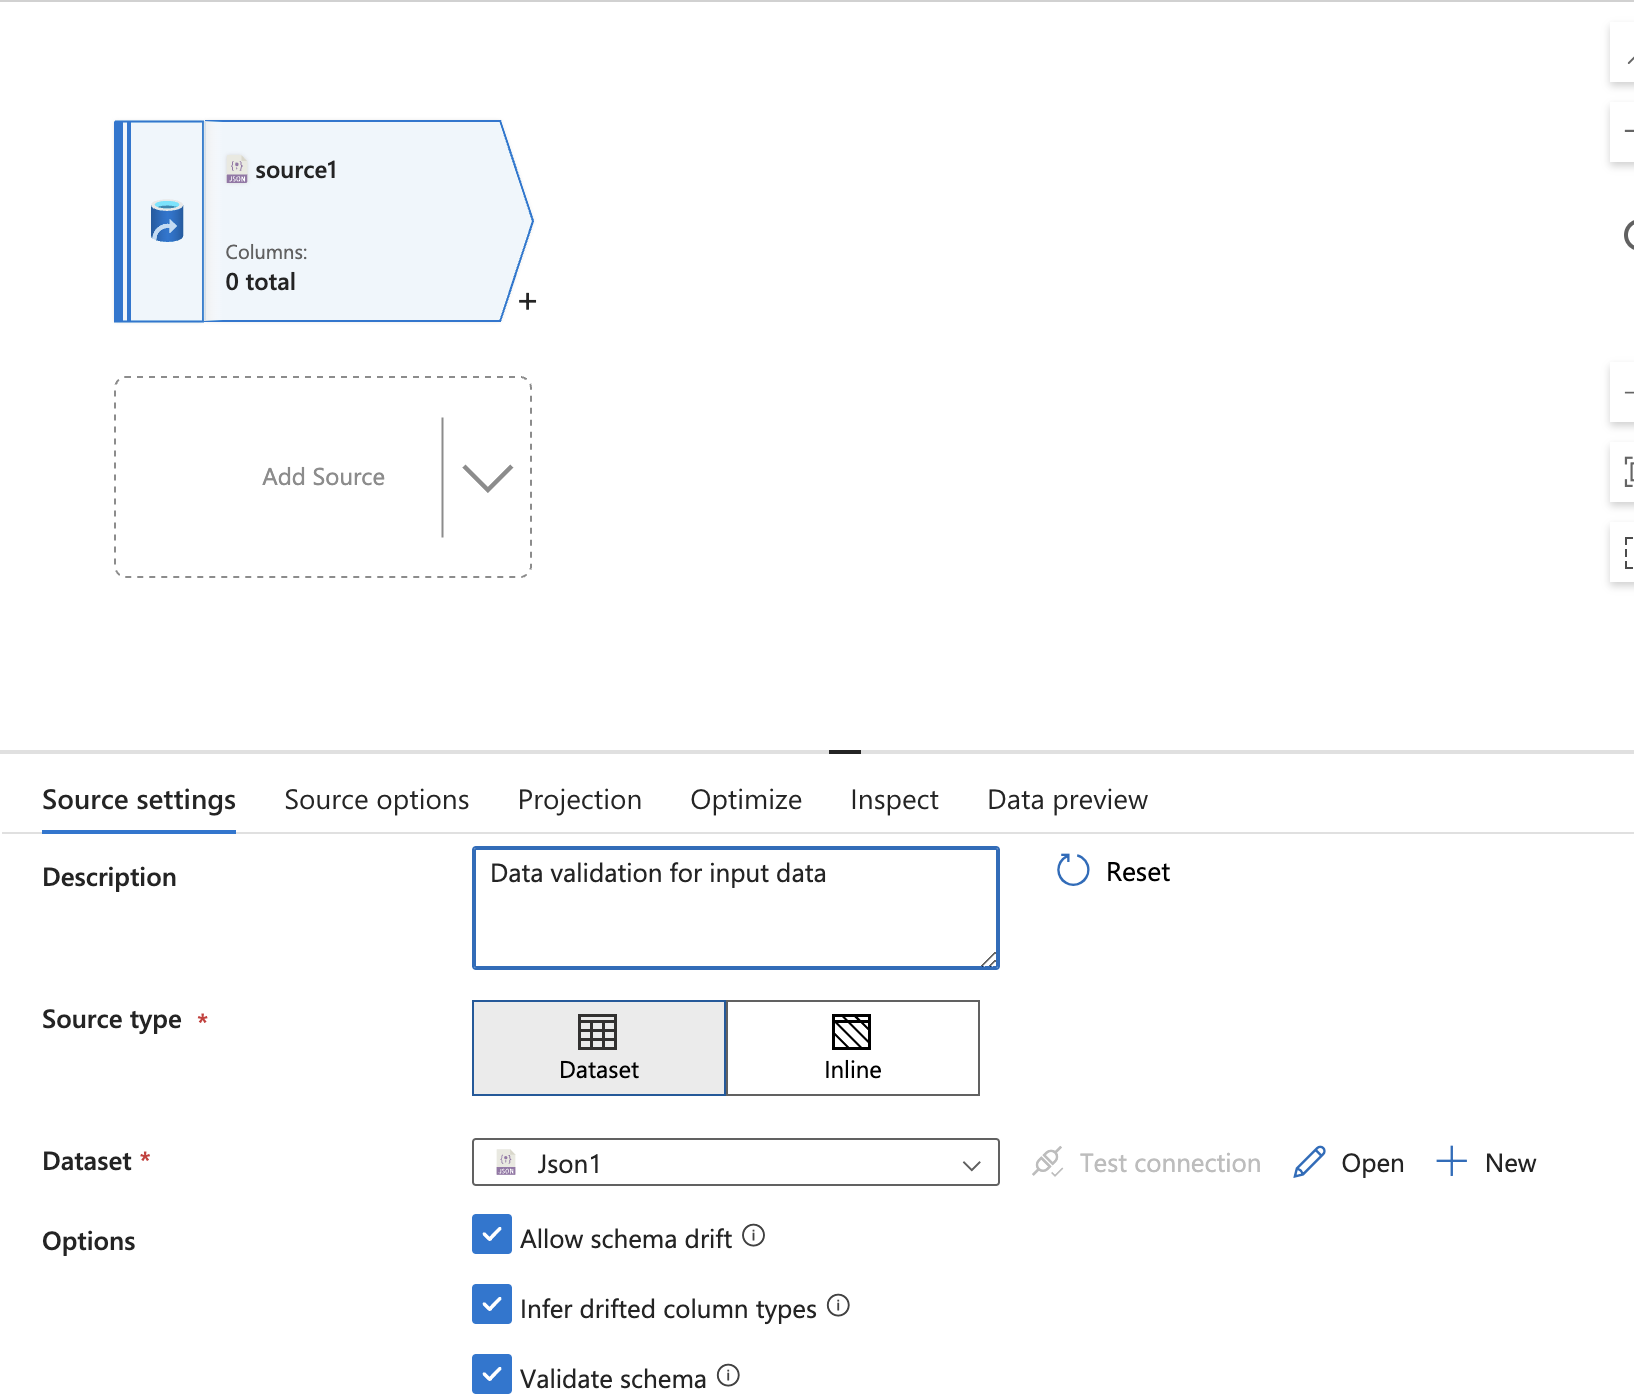
\includegraphics[width=6in]{images/dataflow} 
   \caption{Using data flow for a more in depth data validation}
   \label{fig:dataflow}
\end{figure}


\clearpage


\begin{thebibliography}{9}

\bibitem{threads}
Wikipedia, Threads \href{https://en.wikipedia.org/wiki/Thread_(computing) }{\url{https://en.wikipedia.org/wiki/Thread_(computing)}}

\bibitem{process}
Wikipedia, Processes \href{https://en.wikipedia.org/wiki/Process_(computing)}{\url{https://en.wikipedia.org/wiki/Process_(computing)}}

\bibitem{multiprocess}
Python package Multiprocessing documentation, \href{https://docs.python.org/3/library/multiprocessing.html}{\url{https://docs.python.org/3/library/multiprocessing.html}}



\bibitem{wiki}
Wikipedia, \href{https://en.wikipedia.org/wiki/Data_format }{\url{https://en.wikipedia.org/wiki/Data_format }}

\bibitem{validation}
Microsoft Azure Documentation, \href{https://learn.microsoft.com/en-us/azure/data-factory/control-flow-validation-activity}{\url{https://learn.microsoft.com/en-us/azure/data-factory/control-flow-validation-activity}}

\bibitem{debugtool}
Microsoft Azure Documentation, \href{https://learn.microsoft.com/en-us/azure/data-factory/iterative-development-debugging?tabs=data-factory}{\url{https://learn.microsoft.com/en-us/azure/data-factory/iterative-development-debugging?tabs=data-factory}}

\bibitem{dataflow}
Microsoft Azure Documentation, \href{https://learn.microsoft.com/en-us/azure/data-factory/control-flow-execute-data-flow-activity}{\url{https://learn.microsoft.com/en-us/azure/data-factory/control-flow-execute-data-flow-activity}}

\end{thebibliography}


\end{document}  